\section{Introduction}
\label{sec:intro}
This paper introduces a distributed in-network hash table (DIHT) approach to realize a global scale name resolution service for mobility support in the future Internet. Large-scale in-network global name resolution services under consideration here are motivated by the dramatic growth of mobile devices and applications on the Internet. There are over 6 billion cellular devices in use today with a significant fraction of these providing data services in addition to voice and text. For example, a white paper from Cisco~\cite{cisco} predicts a cross-over of mobile Internet traffic volumes over that of fixed hosts by the year 2015. Current approaches for handling mobility involve a combination of cellular network protocols (e.g. 3GPP)~\cite{3gpp} and mobile IP~\cite{gundavelli} but it is widely recognized that these solutions have serious limitations in terms of scale and service flexibility. This has motivated a number of "clean-slate" future Internet architecture projects aimed at investigating fundamentally new approaches to meeting anticipated needs such as large-scale mobility, security/privacy or content support~\cite{fia}.
\begin{center}
    \begin{figure}[h]
            \vspace{-0.2in}
        \centering
        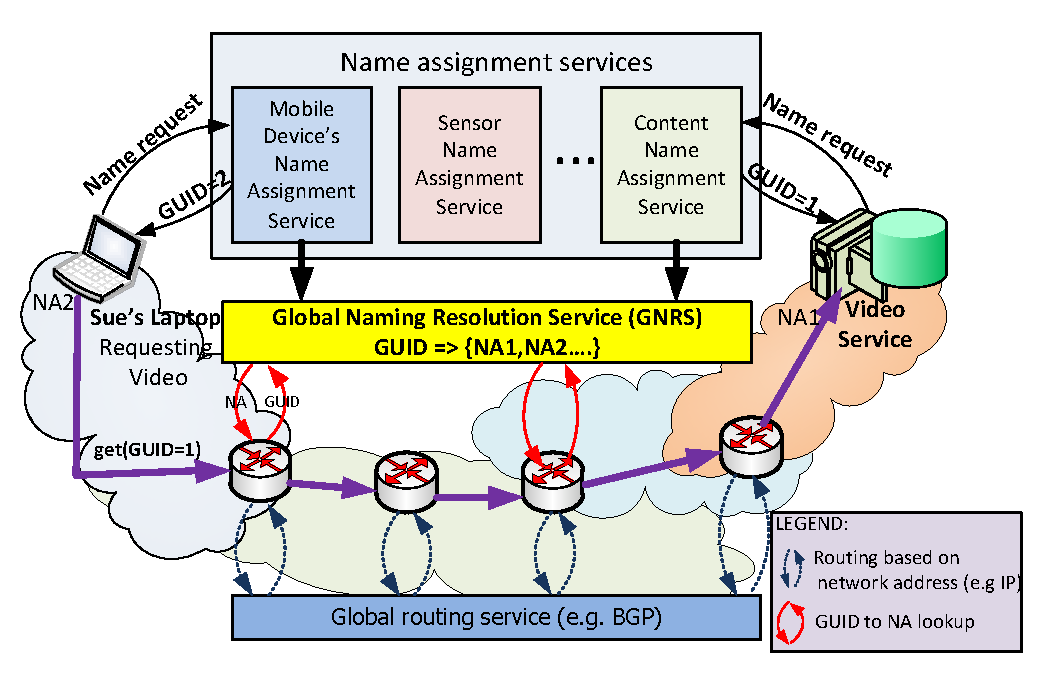
\includegraphics[width=0.5\textwidth]{figures/intro.eps}
        \caption{Global name resolution service concept supporting separation of network names and addresses
    }
        \label{fig:intro}
        \vspace{-0.2in}
    \end{figure}
\end{center}
The MobilityFirst project~\cite{mobilityFirst} represents one of these architectural efforts with a particular focus on supporting large-scale, efficient and robust mobility services in the future Internet. The MobilityFirst architecture (which is still evolving) is based on a clean separation between the ``names" of end-users or other network-connected objects, and their routable addresses or locators. Separation of names and addresses makes it possible for mobile devices to have a permanent, location independent name or globally unique identifier (GUID) which can then be mapped to a set of routable network addresses (NA) corresponding to the current point(s) of attachment. This concept of separating names from addresses has been proposed in earlier work, such as~\cite{farinacci,andersen} but is usually viewed as an overlay service above the network similar in spirit to DNS. The MobilityFirst architecture aims to integrate a global name resolution service (GNRS) as a basic network-layer service which can be efficiently accessed both by end-user devices and in-network routers, base stations and access points. This concept is illustrated in Figure~\ref{fig:intro} which shows the layering of functionality in the proposed MobilityFirst architecture. In this approach, a human-readable name such as ''Sue's laptop" is mapped to a GUID through one of many possible application level services deployed by the network provider or independent third-party providers. The GUID is then assigned to the mobile device (or other network-connected object) and entered into the network-level GNRS service shown in the figure. The GNRS is a distributed network service which is responsible for maintaining the current bindings between the GUID and network address(es) (NA's). Mobile devices (or routers at their point of attachment) update the GNRS with current NA values resulting in a table entry such as $<$GUID: NA1, NA2, NA3, optional properties$>$. The technical problem addressed here is that of realizing a scalable GNRS service with $\sim$10 Billion GUID entries (i.e. network-attached objects) with lookup latencies fast enough to support anticipated mobility speeds and application usage patterns. We emphasize that since the GNRS can also be queried by the in-network routers for dynamic GUID:NA resolution for in-transit packets, low latency in the query response procedure is a critical requirement for the design.

Our approach addresses this problem through an in-network single-hop hashing technique that leverages the IP reachability information readily available at the network layer. It distributes the GUID to address mappings amongst Internet ASs. To look up a mapping, one can directly hash the GUID to produce an IP address of the AS that stores the mapping. Thus, this technique can achieve low lookup latency and minimum maintenance overhead without the need for more churn-tolerant DHTs. While the following sections describe this service in the context of IP, it is flexible enough so that it can also be used with other identifier schemes and addressing structures.
